In this Chapter, we detail the adopted methodology to perform optimal sizing of stand-alone solar PV systems, more specifically using model checking. Diagrams, flowcharts, and algorithms support and explain the solutions.

Besides that, we present all the assumptions and premises adopted. This chapter supports as well the results/conclusions, with direct impact on it. 

It is important to emphasize that the whole explanation about the theoretical basis of the subject discussed here is present in the previous chapter. In addition, we do suggest that previous reading must be done to facilitate the understanding.

\section{Optimal Sizing of Solar PV Systems}

Fig.~\ref{fig:optimization} illustrates how to obtain the optimal sizing of a stand-alone solar PV system, passing through the traditional techniques (manual, and simulation), and including the proposed automatic synthesis that is detailed in this Section. 

One more time, as depicted in automated verification process, the input information is the same for all the methods, with the difference that in automated validation it is possible to define the bound $k$ to restrict the design-space search. And the outputs are not equal, as the design-space coverage and the, mainly, the final resulting.

\begin{figure}[h]
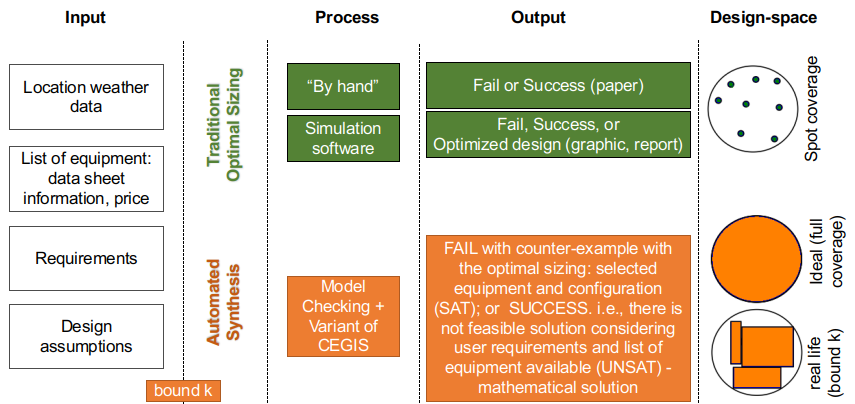
\includegraphics[width=1.0\textwidth]{optimalsizingprocess2}
\centering
\caption{Comparative of optimal sizing methods}
\label{fig:optimization}
\end{figure}
 
\subsection{Variant of CEGIS} 

In Figure~\ref{CEGISalt}, it is pictured a variant of CEGIS previously presented in Section ~\ref{sec:ProgramSynthesis}, Fig.~\ref{Counter-Example-Guided-Inductive-Synthesis}. This variant was created during this Thesis and it will be detailed in this Section.

\begin{figure}[h]
	\centering
	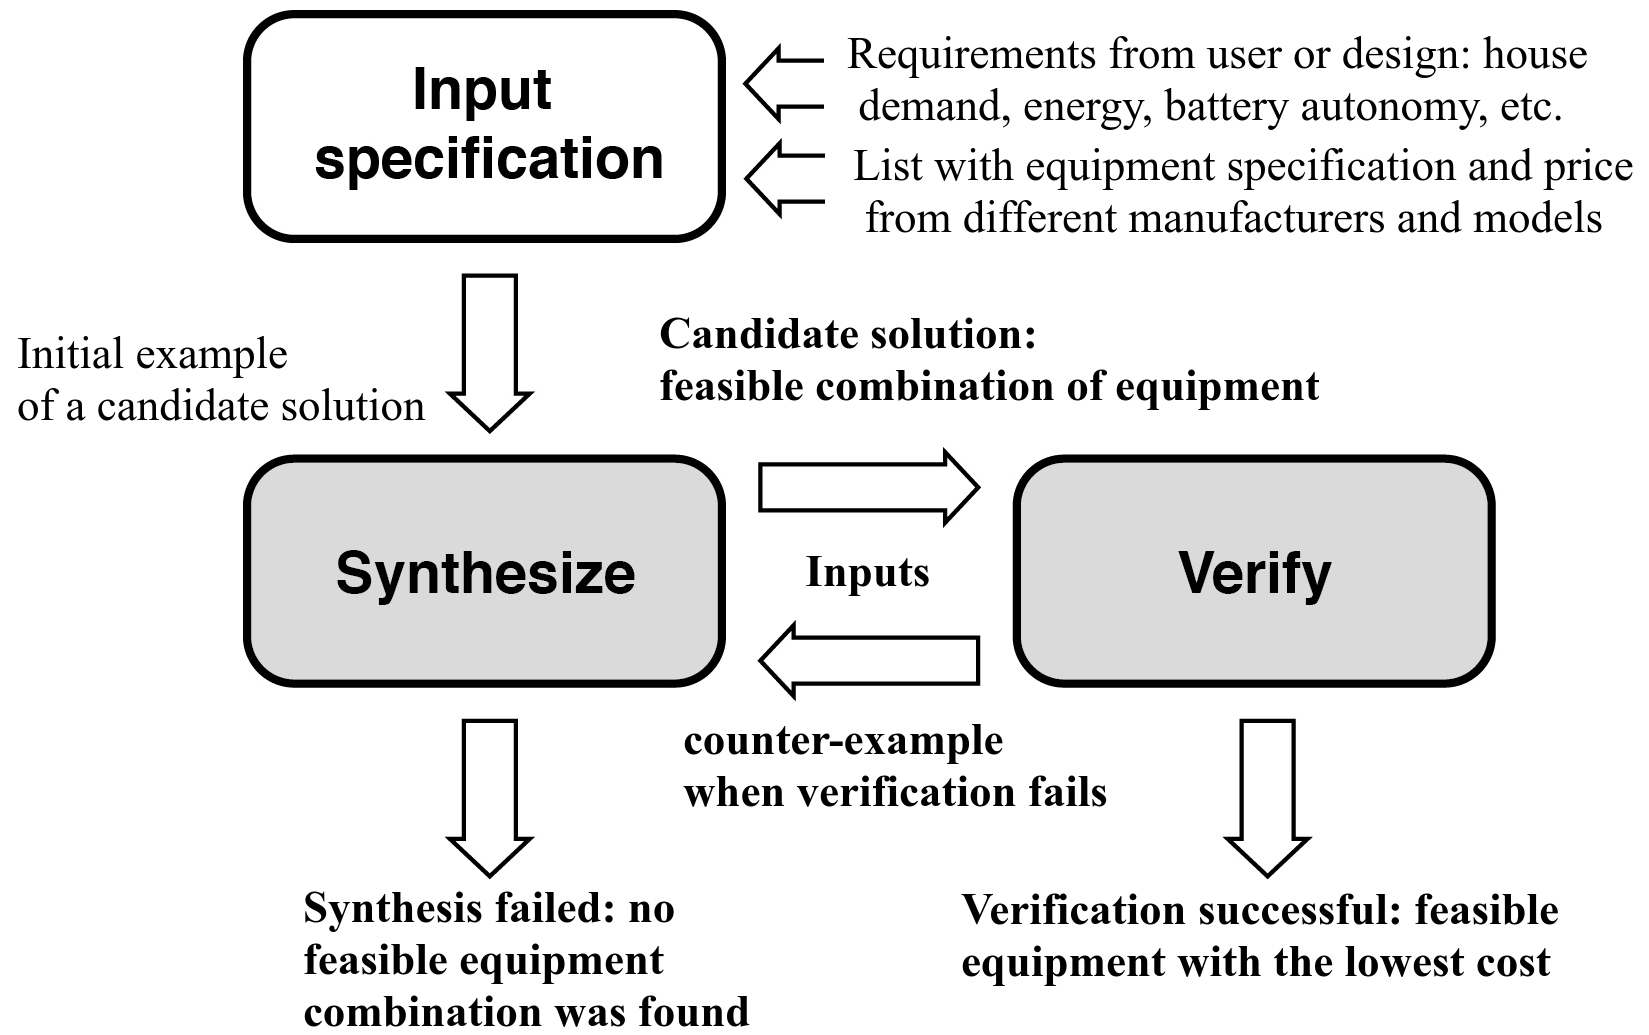
\includegraphics[width=0.75\columnwidth]{fig2_rev.jpg}
	\caption{CEGIS applied to PV system sizing.}
	\label{CEGISalt}
\end{figure}

Examples of specification used by the proposed method include solar insolation (site dependent), house power demand, house consumption energy, estimated load curve, AC voltage, and battery autonomy; we also provide a list of equipment specification and price from different manufacturers and models. Design assumptions are considered project specification as well. The assumptions regarding the optimal sizing are listed in Section~\ref{sec:OptAssumptions}.

There are four particular differences related to the traditional CEGIS described in Figure ~\ref{Counter-Example-Guided-Inductive-Synthesis} when compared to the variant CEGIS used in the proposed approach: 

\begin{itemize}
\item There exists no test vector and every candidate is generated during the run-time in the {\sc Synthesize} phase and sent to the {\sc Verify} phase; 
\item If the {\sc Verify} phase is unsuccessful, then a new candidate is generated by {\sc Synthesize} 
\item The lower bound of the {\sc Verify} phase is incremented to search for the lowest cost; 
\item As a result, there exists no refinement from the {\sc Verify} phase back to the {\sc Synthesize} phase, i.e., a new counterexample is not added to the {\sc input} set since a failure during the {\sc Verify} phase will only discard a given candidate that could be feasible in the next iteration with a new lower bound.
\end{itemize}

Program synthesis engines that implement the CEGIS approach~\cite{sketch} can automatically produce solutions for a large variety of specifications; here we have used symbolic software verifiers based on SMT solvers.

Algorithm~\ref{alg:opt-algorithm} describes our pseudo-code to synthesize stand-alone PV systems using symbolic model checking. It was adopted the analytical method of optimization, with LCC economical analysis and power reliability based on the critical period criteria.
%
 \begin{algorithm}
 \caption{Synthesis algorithm}
 \begin{algorithmic}[1]
 \renewcommand{\algorithmicrequire}{\textbf{Input:}}
 \renewcommand{\algorithmicensure}{\textbf{Output:}}
  \STATE Initialize variables \\
  \STATE Declare list of PV panels, controllers, batteries, and inverters data and cost \\
%  \STATE Declare list of controllers data and cost \\
%  \STATE Declare list of batteries data and cost \\
%  \STATE Declare list of inverters data and cost \\
  \STATE Declare the maximum possible cost $MaxCost$  \\
  \STATE Declare power demand, power peak, energy consumption \\
  \STATE Declare battery autonomy, deep of discharge, AC voltage \\
  \FOR {$HintCost=0$ to $MaxCost$}
 	\STATE Declare non-deterministic variable to select PV Panel from list \\
 	\STATE Declare non-deterministic variable to select Controller from list \\
 	\STATE Declare non-deterministic variable to select Battery from list \\
 	\STATE Declare non-deterministic variable to select Inverter from list \\ 	
 	\STATE Calculate $E_{corrected}, \, E_{p} $ \\
	\STATE Calculate $N_{TPmin}, \, N_{PSmin}, N_{PPmin} $ \\
 	\STATE Calculate $C_{bank}$ \\
	\STATE Calculate $N_{BS}min, \, N_{BP}min, \, N_{B}total$ \\
	\STATE Requirement enforced by \textbf{assume}$(V_{c})$ \\
 	\STATE Calculate $I_{sc,amb}$ \\
 	\STATE Calculate $I_{c,min}$ \\
 	\STATE Requirement enforced by \textbf{assume}$(I_{c} \wedge V_{in}DC \wedge V_{out}AC)$ \\
%	\STATE Requirement enforced by \textbf{assume}$(V_{in}DC \wedge V_{out}AC )$ \\
%	\STATE Requirement enforced by \textbf{assume}$(V_{out}AC)$ \\
	\STATE Requirement enforced by \textbf{assume}$(Demand \wedge P_{surge})$ \\
%	\STATE Requirement enforced by \textbf{assume}$(P_{surge})$ \\
	\STATE non-deterministic variables hold feasible equipment and cost  \\
	\STATE $F_{obj} \leftarrow  N_{TP}*Panel_{Cost} \, + \, N_{TB}*Battery_{Cost} \, + Controller_{Cost} \, + \, Inverter_{Cost} \, + \, Installation_{Cost} \, + \, batrep_{Cost} \, + \, PWO\&M_{Cost}$ \\
	\STATE Violation check with \textbf{assert}$(F_{obj} > HintCost)$ \\
  \ENDFOR
 \RETURN $(\,)$ 
 \end{algorithmic} 
 \label{alg:opt-algorithm}
 \end{algorithm}
%

Our synthesis algorithm will synthesize constant values; 
it starts with the input of manufacturers data and prices of PV panels, batteries, 
charge controllers and inverters (line $2$). After that, we define user requirements, i.e., 
house requirements and design definitions, from lines $4$ and $5$. 

The \textit{for}-loop started at line $6$ controls the lowest cost to the PV solution. 
In particular, it starts with cost $0$ and stops only when the algorithm finds a 
feasible solution in which the cost breaks the $assertion$ stated in line $22$; 
if that happens, then our algorithm has found an optimal solution, thereby stating 
that the {\sc Verify} phase reached a satisfiable condition (\textit{SAT}). 
The $MaxCost$ value at line $6$ is just a very high value put as a limit 
to the \textit{for}-loop, that never will be reached because the optimal solution will be found first.

Our synthesis algorithm uses non-deterministic variables to choose one specific constant 
from a given list of PV panels, controllers, batteries and inverters (lines $7$ to $10$). 
That procedure ensures that our synthesis engine checks all combinations of items 
from each equipment, and combine them to assemble a feasible (candidate) PV solution, 
which meets the user requirements.

Next, we use Eq.~\eqref{eq:Ecorrected}, Eq.~\eqref{eq:Ep}, Eq.~\eqref{eq:NTPmin}, 
Eq.~\eqref{eq:NPSmin}, Eq.~\eqref{eq:NPPmin}, Eq.~\eqref{eq:Cbank}, 
Eq.~\eqref{eq:Nbtotal}, Eq.~\eqref{eq:iscamb}, and Eq.~\eqref{eq:icmin} to calculate the sizing variables (lines $11$ to $17$). The directive \textit{assume} (lines $15$, $18$ and $19$) 
ensures the compatibility of the chosen items from the list of equipment: the {\sc Verify} phase 
uses only the item (among all the possible ones) that satisfies the statements of Lines $15$, $18$ and $19$. Line $15$ is specific to the charge controller voltage check. Line $18$ checks the inverter check $I_{c}$, charge controller DC input voltage $V_{in}DC$, and charge controller AC output voltage $V_{in}DC$ check. Line $19$ ensures the power demand and the surge power of inverter.
Therefore, our synthesis algorithm reaches line $20$ with one feasible solution, 
and the cost of that solution is calculated in $F_{obj}$ (line $21$). This cost is the equivalent of ~\ref{eq:LCC} described in Section ~\ref{sec:optcriteria}.

If our algorithm does not find a feasible solution among the item of equipment that 
were provided to our {\sc Synthesize} phase,  then the result is an unsatisfiable (\textit{UNSAT}), i.e., 
the program finishes and does not find a solution, which indicates that it 
was not possible to combine the items of each equipment in order to create a feasible solution. 

The main challenge for the {\sc Synthesize} phase is to find a feasible candidate 
solution regarding the constraints and user requirements. Related to our {\sc Verify} 
phase the challenge is to find the lowest acquisition cost from a list of equipment and 
components that is provided from the {\sc Synthesize} phase. 

Note that the process described here is completely automated and that a validation is performed 
by our {\sc Verify} phase to ensure that the approach is sound.

\subsection{Optimization Assumptions and Premises}
\label{sec:OptAssumptions}
%%%%%%%%%%%%%%%%%%%%%%%%%%%%%%%

Here some premise are presented and some adopted assumptions are explained for the optimal sizing method, regarding the automated synthesis and simulation software.

Regarding the line $2$ of Algorithm~\ref{alg:opt-algorithm}, 
a list of forty equipment from ten different manufacturers was provided 
to the synthesis engine in order to allow the choice of every item 
of PV sizing. Data sheet from each item was necessary to collect 
technical information. Moreover, the price of each item was obtained 
from available quotations in the market, and if the currency was not in US dollars, 
then it was used the exchange rate of the day to convert it to US dollars.

With respect to power reliability, this work will rely on the critical period solar 
energy method~\cite{Pinho} as described in Section~\ref{sec:sizing}. 
The usual way is to use loss of load probability (LOLP) or loss of power 
supply probability (LPSP). However, based on the fact that here we 
are neither considering site characteristics nor the load changes over time, 
which demands historical data, the reliability analysis will be developed only 
by the critical period method of PV sizing.

Regarding financial analysis:
\begin{itemize}
	\item LCC lifetime considered: $20$ years;
	\item Installation costs: includes delivery in the isolated community and installation costs itself, $5$\% of total cost~\cite{Agrener2013};
	\item Value of the discount rate or interest rate: $10$\%, which is a good rate considering financial investments in developing countries;
	\item Operation and maintenance annual costs: based on past PV projects of similar size in the Amazon region of Brazil, will be adopted the value of US\$ 289.64~\cite{Agrener2013}. This cost includes the battery replacement based on its lifetime ($4$ years for lead-acid batteries), plus inverters and controller replacement (every $10$ years). Therefore, it will be performed three battery bank and one inverter-controller replacements during the LCC analysis.
\end{itemize}

On the subject of PV system optimization technique, we will adopt here the intuitive method 
since the average value daily of solar irradiance is used in the mathematical model, 
without considering the battery's state of charge, or even the random nature 
of solar irradiation and meteorological conditions. Therefore, all the computational 
effort will be concentrated in our automated synthesis algorithm.

Regarding batteries, the voltage of the system (DC bus) is set in $24$ V DC (but the value can be adjusted to $12$ or $48$ V at the code).

Related to HOMER Pro:

\begin{itemize}
	\item HOMER Pro do not have the LCC cost in its reports. However, it has NPC and LCOE. Therefore NPC was used to obtain LCC in order to allow the comparative among tools;
	\item The optimization analysis of HOMER Pro allows to define a load curve and temperature according of data collected automatically from online databases. However, in order to allow a correct comparative, the curve load and the temperature were defined exactly the same as automated synthesis tools;
	\item Battery autonomy is not an parameter that the user can set when using HOMER Pro. The tool will always to meet the user requirement, i.e., the load curve during the $365$ days of the year;
	\item HOMER Pro do not have a explicit equipment called charge controller. It uses a controller resource that can perform in two different ways, according of the optimization choice or the user choice: load following or cycle charging~\cite{HOMER}. During the tests it was chosen the load following controller: it produces only enough power to meet the demand~\cite{HOMER};
	\item It was assumed the value of 5\% of capacity shortage that is equivalent to 95\% of availability of the PV system. By definition, availability is the percentage of time at which a power system is capable of meeting the load requirements~\cite{Khatib2014}. For critical loads, 99\% is considered acceptable. While in a ordinary house electrical load, 95\% is considered acceptable;
	\item It was assumed a string of two batteries in order to match the voltage of the system of $24$ V DC that was used for the automated synthesis tool;
	\item The premise adopted when using HOMER Pro it was that the user does not know the optimal solution, and that in order to obtain this solution is necessary to include (at the design phase of the tool) generic PV and batteries modules that HOMER Pro will search for the optimized power of each component. With that in mind, it was included a generic flat plate PV of $1$ kW and generic lead-acid batteries of $1$ kW as well (and with capacity of $83.4$ Ah according with HOMER Pro modeling). HOMER, during run-time, decides the size in kW of each module, based on feasibility and lower cost.
\end{itemize}

\section{General Assumptions}

The general assumptions for the scientific method of automated synthesis are the same presented at Chapter~\nameref{chap:methodology1}, related to the code in ANSI-C, to the bound $k$, to simulation tool comparative, and to the battery state of charge.


\section{Conclusion}

In this Chapter we showed in details how the state-of-art computer science method of automated synthesis method was adapted in order to be used in stand-alone solar PV systems to obtain the optimal project sizing. Moreover, is was possible to picture how the proposed method compares with the traditional use of simulation tool for the same purpose.

Detailed diagrams, flowcharts and algorithms with pseudo-code were presented with the aim to support the proposed work and to facilitate the understanding. And even more so, the assumptions adopted for the automated verification and simulation software were listed, because those assumptions have impact at the results there will be presented at  \autoref{chap:automatedsynthesis}. 

